\subsection{COWCat}

\begin{frame}
  {Taxonomie für Webdokument-Klassifikation}
  \begin{itemize}
    \item EAGLES/Sharoff-basiert
    \item multiple Dimensionen, keine Genres
    \item nur Kategorien mit potentiellem Einfluss\\auf grammatische Kategorien 
    \item Aim, Audience, Authorship, Domain, Mode
  \end{itemize}
\end{frame}

\begin{frame}
  {Experiment zum Deutschen}
  \begin{itemize}
    \item 4 Rater
    \item 800 Dokumente
    \item Trainingphase: 100 Dokumente, 2 Treffen
  \end{itemize}
\end{frame}

\begin{frame}
  {Ergebnisse: Deutsch}
  Agree and $\kappa$ (Cohen) für die zwei Rater mit der jeweils besten Übereinstimmung
  \vspace{0.5cm}
  \begin{center}
    \begin{tabular}[h]{lrrrr}
      \hline
      & Aim (5) & Aud (3) & Auth (5) & Mode (4) \\
      \hline
      \hline
      Agree & 0.82 & 0.77 & 0.78 & 0.92 \\
      $\kappa$ & 0.58 & 0.53 & 0.71 & 0.82 \\
      \hline
    \end{tabular}
  \end{center}
\end{frame}

\begin{frame}
  {Ergebnisse: Spanisch}
  Sind vielleicht die Hilfskräfte schuld?\\
  Hier die Ergebnisse für Lea Helmers und Felix Bildhauer:\\ 
  \vspace{0.5cm}
  \begin{center}
    \begin{tabular}[h]{lrrrr}
      \hline
      & Aim (5) & Aud (3) & Auth (5) & Mode (4) \\
      \hline
      \hline
      Agree & 0.73 & 0.87 & 0.71 & 0.94 \\
      $\kappa$ & 0.49 & 0.21 & 0.55 & 0.64 \\
      \hline
    \end{tabular}
  \end{center}
  \pause
  \vspace{0.5cm}
  Klar \textbf{schlechter}!
\end{frame}

\begin{frame}
  {Konfusion: Aim (Spanisch)}
  \vspace{0.5cm}
  \begin{center}
    \scalebox{0.8}{
      \begin{tabular}[h]{r|rrrrr}
	&  Di & Fi&  If & Is & Re\\
	\hline
      Di& 253 &  0&  20 &  4 &  2\\ 
      Fi&   0 &  2&   0 &  0 &  0\\ 
      If&  78 &  0&  92 &  6 &  2\\ 
      Is&  10 &  0&   2 &  8 &  0\\ 
      Re&   7 &  0&   1 &  2 & 10\\ 
      \end{tabular}
    }
  \end{center}
\end{frame}

\begin{frame}
  {Konfusion: Audience (Spanisch)}
  \vspace{0.5cm}
  \begin{center}
    \scalebox{0.8}{
      \begin{tabular}[h]{r|rrr}
        &  Ge & In & Pr \\ 
	\hline
      Ge& 426 & 32 &  9 \\ 
      In&  15 &  5 &  4 \\ 
      Pr&   4 &  1 &  4 \\ 
      \end{tabular}
    }
  \end{center}
\end{frame}

\begin{frame}
  {Konfusion: Authorship (Spanisch)}
  \vspace{0.5cm}
  \begin{center}
    \scalebox{0.8}{
      \begin{tabular}[h]{r|rrrrr}
        &  Co & Mu & Sf & Sm&  Un \\ 
	\hline
      Co&  40 &  0 &  1 &  5&  18 \\ 
      Mu&   0 & 37 &  0 &  4&  12 \\ 
      Sf&   0 &  0 & 19 &  1&   4 \\ 
      Sm&   0 &  2 &  1 & 42&  11 \\ 
      Su&   0 &  1 &  3 &  6&  18 \\ 
      Un&  12 & 14 &  9 & 24& 216 \\ 
      \end{tabular}
    }
  \end{center}
\end{frame}

\begin{frame}
  {Konfusion: Mode (Spanisch)}
  \vspace{0.5cm}
  \begin{center}
    \scalebox{0.8}{
      \begin{tabular}[h]{r|rrrr}
         & Bm & Qs & Sp &  Wr \\
	 \hline
      Bm & 11 &  4 &  0 &   8 \\ 
      Qs &  3 &  6 &  1 &   4 \\ 
      Sp &  0 &  0 &  8 &   3 \\ 
      Wr &  2 &  3 &  2 & 445 \\ 
      \end{tabular}
    }
  \end{center}
\end{frame}

\begin{frame}
  {TLD-Vergleich}
  \centering
  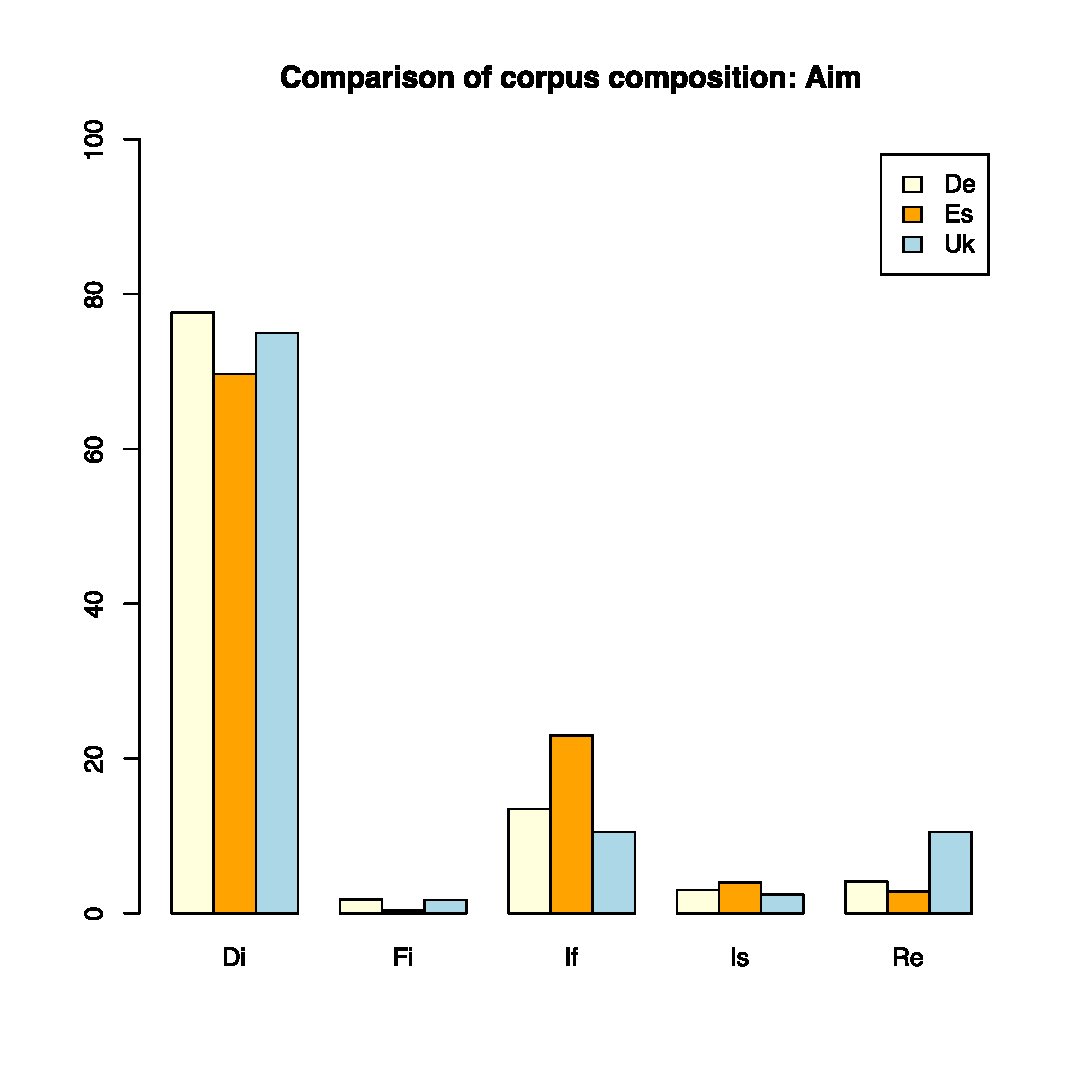
\includegraphics[width=0.65\textwidth]{graphics/aim}
\end{frame}

\begin{frame}
  {TLD-Vergleich}
  \centering
  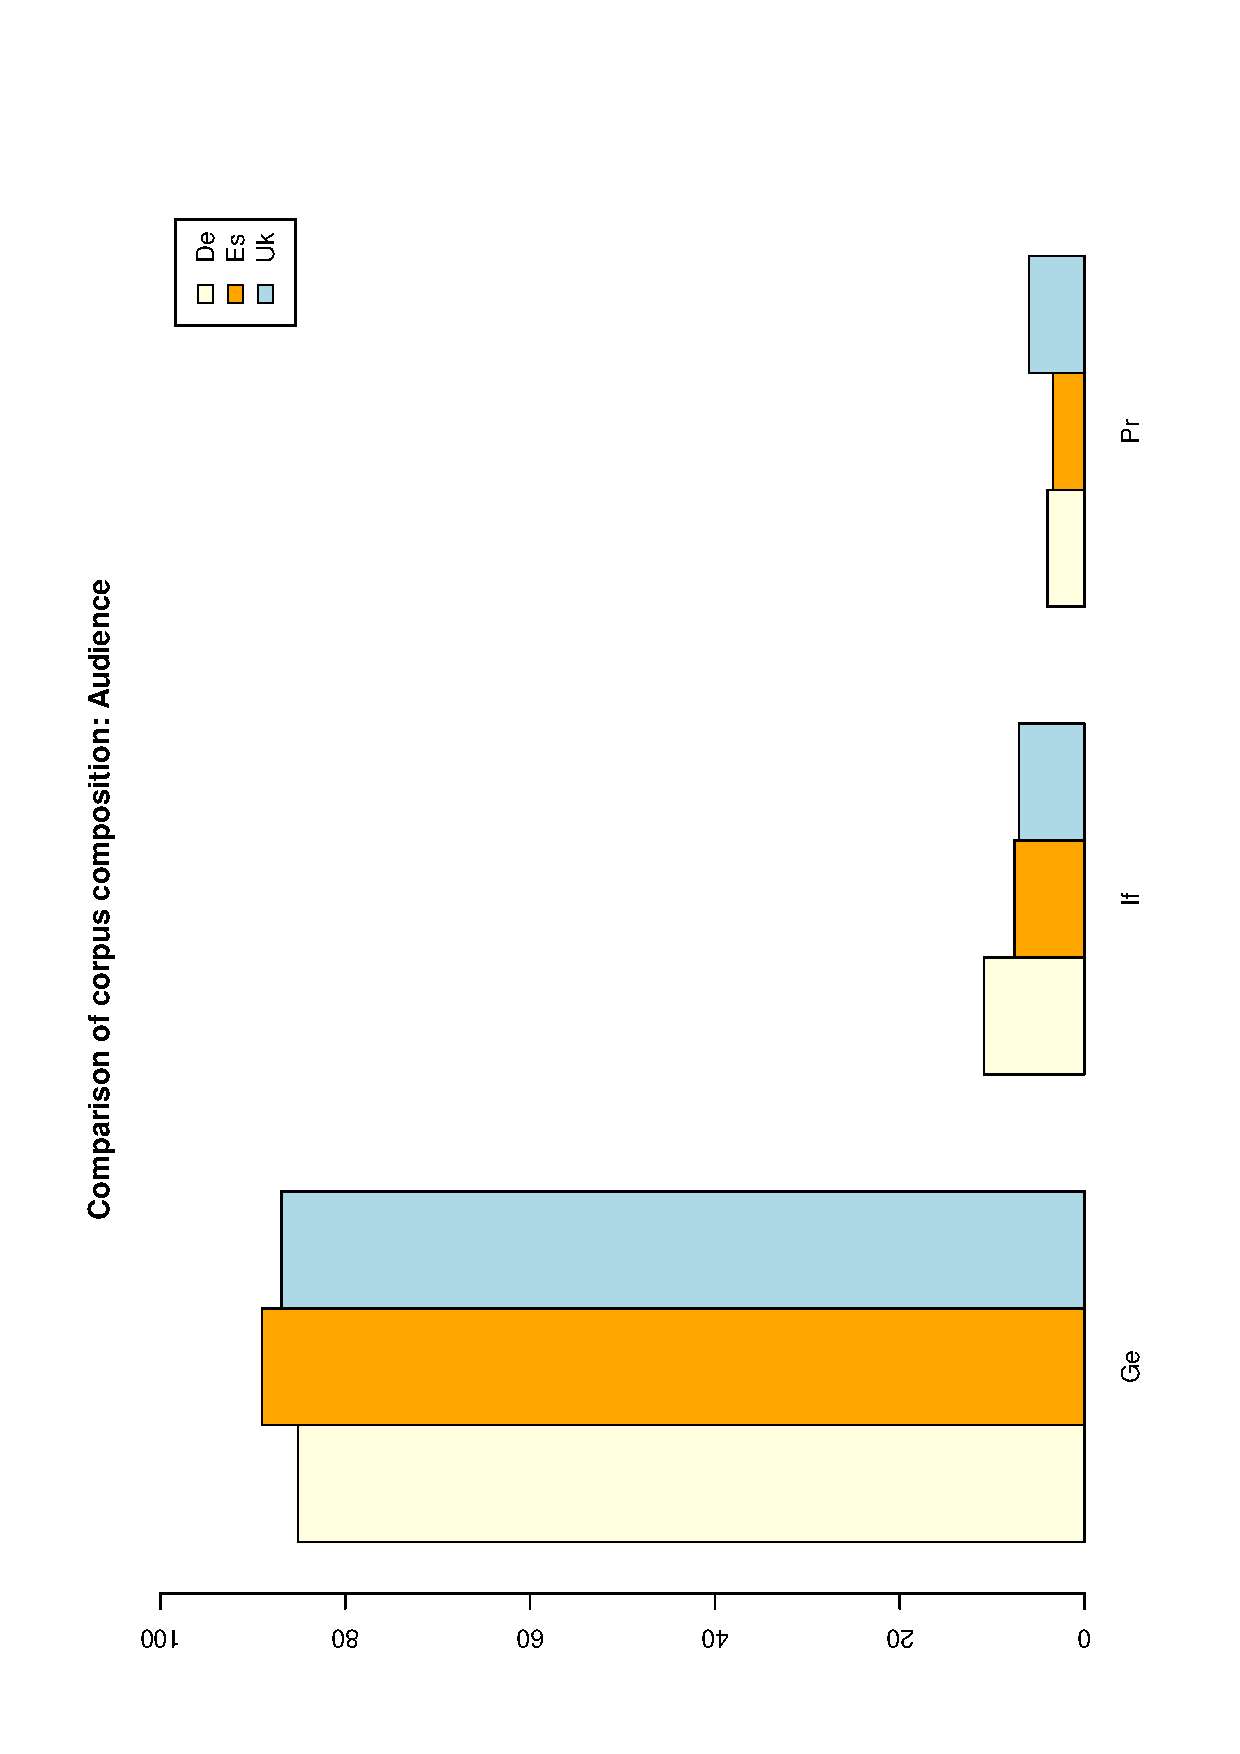
\includegraphics[height=0.95\textheight,angle=270]{graphics/aud}
\end{frame}

\begin{frame}
  {TLD-Vergleich}
  \centering
  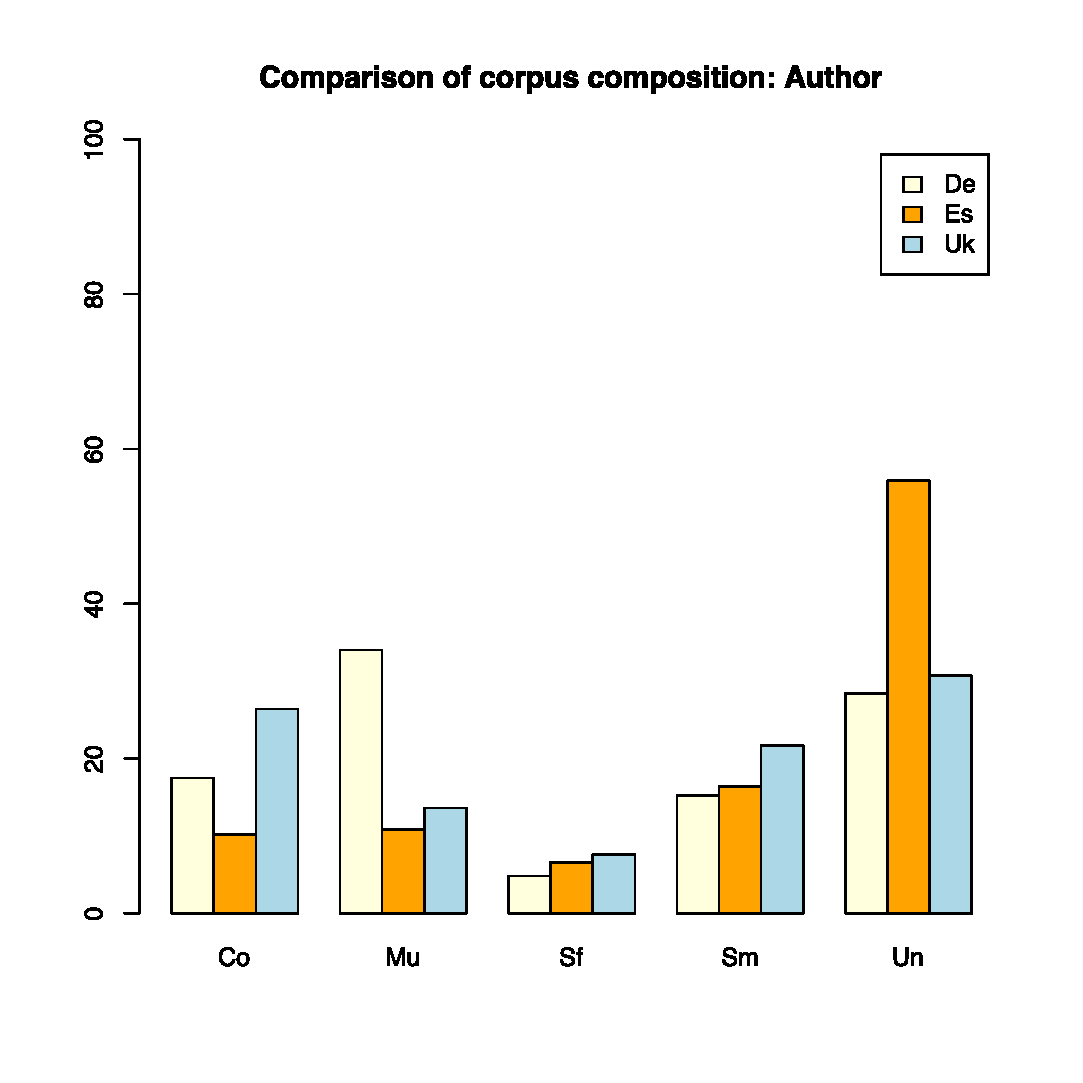
\includegraphics[width=0.65\textwidth]{graphics/aut}
\end{frame}

\begin{frame}
  {TLD-Vergleich}
  \centering
  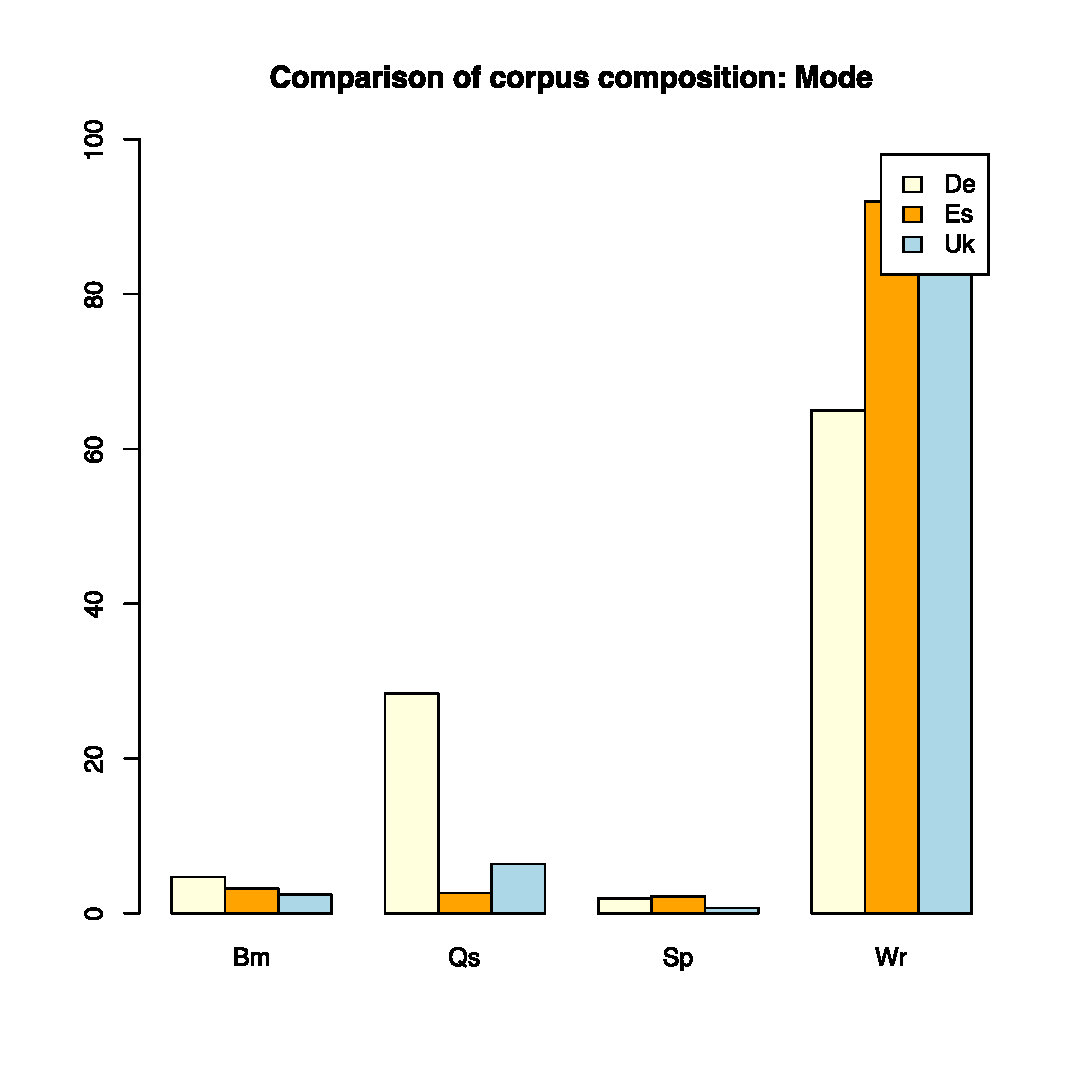
\includegraphics[width=0.65\textwidth]{graphics/mode}
\end{frame}

